\section{Konzept}

\subsection{Use Case Diagramme}
Im folgenden Abschnitt werde ich die Use-Cases identifizieren und beschreiben.\\
Dies dient zum einen zum Erfassen der benötigten Klassen und zum anderen um ein gutes Testkonzept zu erstellen.
 
%---OVERVIEW USECASE-IMAGE---
\subsubsection{Use Case Übersicht}
\begin{figure}[H]
    \begin{center}
      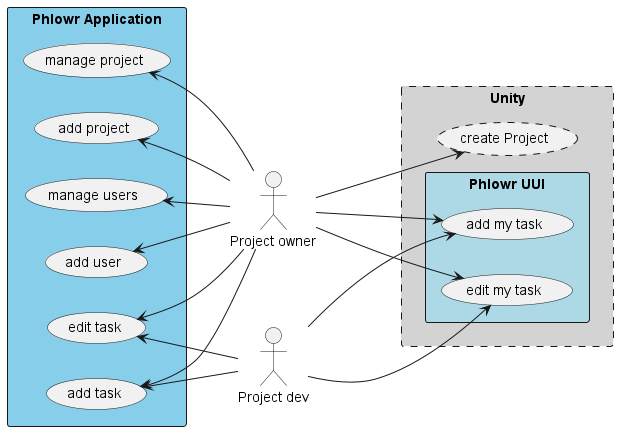
\includegraphics[width=1\linewidth]{../content/diagrams/usecase/overview/overviewUseCase.png}
      \caption{Use Case Diagramm <Übersicht>}
    \end{center}
  \end{figure}

  \newpage
  %---ADD PROJECT USECASE---
\subsubsection{Projekt hinzufügen}
\begin{figure}[H]
  \begin{center}
    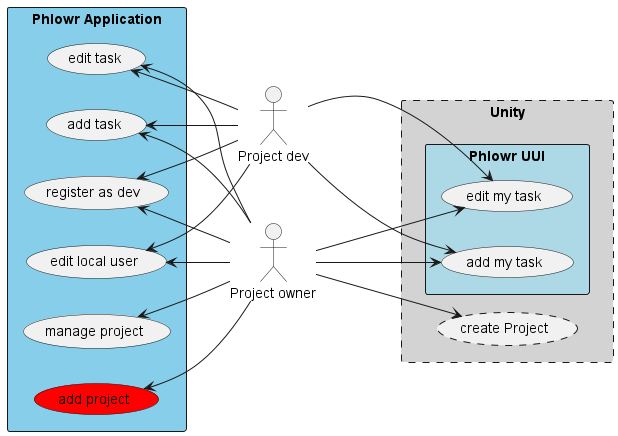
\includegraphics[width=0.3\linewidth]{../content/diagrams/usecase/overview/overviewUseCaseAddProjectSelected.png}
    \caption{Use Case Diagaramm <add project> }
  \end{center}
\end{figure}


\begin{table}[H]
    \centering
    \settowidth\tymin{executeIncomingCommand()}
    \setlength\extrarowheight{2pt}
    \begin{tabulary}{1.0\textwidth}{|m{4cm}|m{10cm}|}
      \hline
      \textbf{Use Case} &
      \textbf{ADD PROJECT}\\
      \hline
      \textbf{Beschreibung} &
      Ein Unity-Projekt wird der Applikation hinzugefügt\\ 
      \hline
      \textbf{Includes} &
      \begin{itemize}
        \item keine 
      \end{itemize}\\ 
      \hline
      \textbf{Akteure} &
      \begin{itemize}
        \item Project Owner
      \end{itemize}\\ 
      \hline
      \textbf{Auslöser} &
      \begin{itemize}
        \item Ein bestehendes Unity-Projekt soll mit Phlowr verwaltet werden
      \end{itemize}\\ 
      \hline
      \textbf{Vorbedingungen} &
      \begin{itemize}
        \item Das hinzuzufügende Unity-Projekt wurde bereits erstellt
      \end{itemize}\\ 
      \hline
      \textbf{Abschlussbedingungen} &
      \begin{itemize}
        \item Das gewünschte Projekt ist in der Applikation erfasst
      \end{itemize}\\ 
      \hline
      \textbf{Ablauf} &
      \begin{enumerate}
        \item Applikation öffnen
        \item <Projekt Hinzufügen> wählen
        \item Den entsprechenden Projekt-Ordner auswählen
        \item Speichern
        \end{enumerate}\\ 
      \hline
      \textbf{Zu Beachten / Notizen} &
      \begin{itemize}
        \item Projekt sollte nur einmal hinzugefügt werden können
        \item Projekt Ordner-Struktur sollte überprüft werden
        \end{itemize}\\ 
      \hline
    \end{tabulary}
    \caption{Use Case: ADD PROJECT}
  \end{table}

\newpage
    %---MANAGE PROJECT USECASE---
\subsubsection{Projekt verwalten}
\begin{figure}[H]
  \begin{center}
    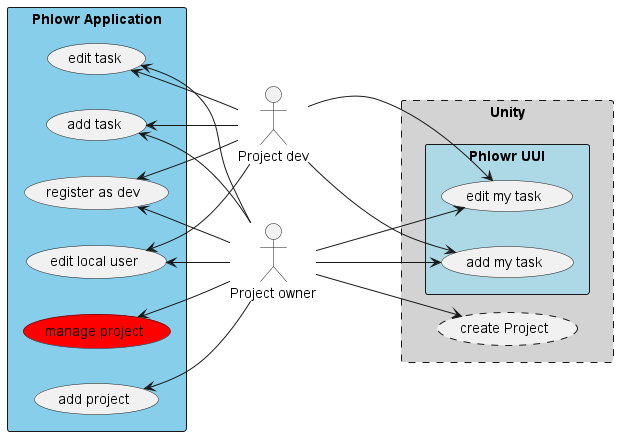
\includegraphics[width=0.3\linewidth]{../content/diagrams/usecase/overview/overviewUseCaseManageProjectSelected.png}
    \caption{Use Case Diagaramm <manage project> }
  \end{center}
\end{figure}

\begin{table}[H]
    \centering
    \settowidth\tymin{executeIncomingCommand()}
    \setlength\extrarowheight{2pt}
    \begin{tabulary}{1.0\textwidth}{|m{4cm}|m{9cm}|}
      \hline
      \textbf{Use Case} &
      \textbf{MANAGE PROJECT}\\
      \hline
      \textbf{Beschreibung} &
      Ein Projekt wird in der applikation verwaltet\\ 
      \hline
      \textbf{Includes} &
      \begin{itemize}
        \item Beschreibung anpassen (edit description)
        \item Name anpassen (edit name)
        \item User-Slots anpassen (edit user-slots)
        \item Projekt-Owner ändern (change PO)
        \end{itemize}\\ 
      \hline 
      \textbf{Akteure} &
      Projekt-Owner\\ 
      \hline
      \textbf{Auslöser} &
      Ein Projekt soll angepasst werden\\ 
      \hline
      \textbf{Vorbedingungen} &
      Das Projekt wurde der Applikation hinzugefügt und der ausführende User ist der Project-Owner\\ 
      \hline
      \textbf{Abschlussbedingungen} &
      Die gewünschten Änderungen wurden gemacht und das Projekt wurde gespeichert\\ 
      \hline
      \textbf{Ablauf} &
      \begin{enumerate}
        \item Applikation öffnen
        \item <Projekt Editieren> wählen
        \item Gewünschte Änderungen vornehmen (siehe Includes)
        \item Speichern
        \end{enumerate}\\ 
      \hline
      \textbf{Zu Beachten / Notizen} &
      \begin{itemize}
        \item Projekte dürfen nur vom PO editiert werden können
        \end{itemize}\\ 
      \hline
    \end{tabulary}
    \caption{Use Case: MANAGE PROJECT}
  \end{table}
 \newpage

\subsubsection{Includes von „Projekt verwalten“}
  \begin{figure}[H]
    \begin{center}
      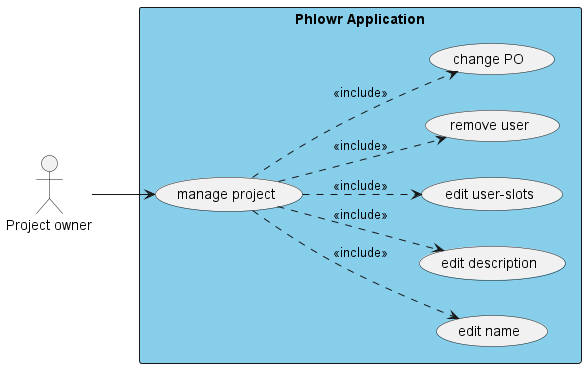
\includegraphics[width=1\linewidth]{../content/diagrams/usecase/manageProject/manageProjectUseCase.png}
      \caption{Use Case Diagaramm <manage project>}
    \end{center}
  \end{figure}

  \newpage
  %---MANAGE Project includes---

   %---CHANGE PO USECASE include---
  \begin{figure}[H]
  \begin{center}
    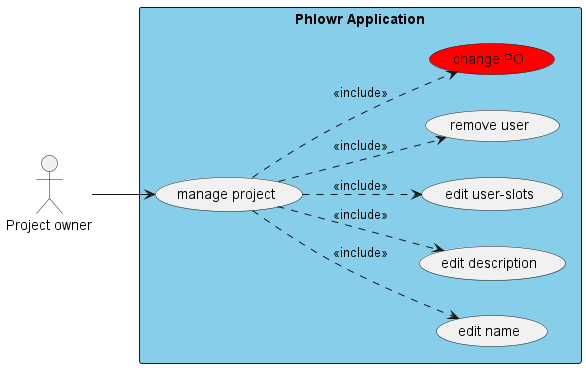
\includegraphics[width=0.3\linewidth]{../content/diagrams/usecase/manageProject/manageProjectUseCaseChangePOSelected.png}
    \caption{Use Case Diagaramm <change PO> }
  \end{center}
\end{figure}


\begin{table}[H]
    \centering
    \settowidth\tymin{executeIncomingCommand()}
    \setlength\extrarowheight{2pt}
    \begin{tabulary}{1.0\textwidth}{|m{4cm}|m{9cm}|}
      \hline
      \textbf{Use Case} &
      \textbf{CHANGE PO}\\
      \hline
      \textbf{Beschreibung} &
      Der Projekt-Owner des Projektes wird geändert\\ 
      \hline
      \textbf{Includes} &
      \begin{itemize}
       \item keine
        \end{itemize}\\  
        \hline
      \textbf{Akteure} &
      Projekt-Owner\\ 
      \hline
      \textbf{Auslöser} &
      Der Projekt-Owner soll geändert werden\\ 
      \hline
      \textbf{Vorbedingungen} &
      \begin{itemize}
        \item Vorbedingungen vom <MANAGE PROJECT>-Use-Case
        \item Der neue Projekt-Owner muss als User im Projekt registriert sein
      \end{itemize}\\  
      \hline
      \textbf{Abschlussbedingunen} &
      Der Projekt-Owner wurde geändert und die Änderungen sind gespeichert\\ 
      \hline
      \textbf{Ablauf} &
      \begin{enumerate}
        \item Applikation öffnen
        \item <Projekt Editieren> wählen
        \item <Change Project Owner> wählen
        \item Neuer PO aus liste der registrierten User auswählen
        \item Speichern
        \end{enumerate}\\ 
      \hline
      \textbf{Zu Beachten / Notizen} &
      \begin{itemize}
        \item Wird ein PO inaktiv, so kann das Projekt nicht mehr bearbeitet werden,
        der PO muss dann manuell im JSON-File geändert werden
        \end{itemize}\\ 
      \hline
    \end{tabulary}
    \caption{Use Case: manage project -> CHANGE PO}
  \end{table}

  \newpage
  
   %---EDIT USER-SLOTS USECASE include---
   
\begin{figure}[H]
    \begin{center}
      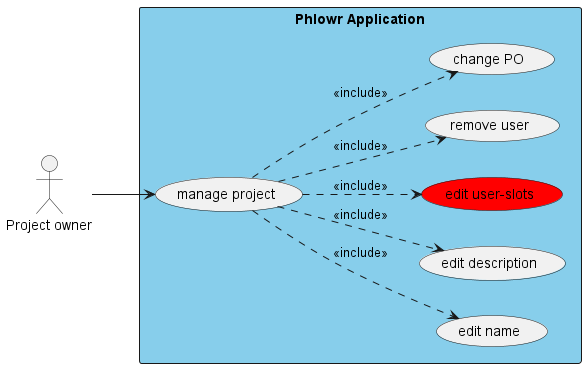
\includegraphics[width=0.3\linewidth]{../content/diagrams/usecase/manageProject/manageProjectUseCaseEditUserSlotsSelected.png}
      \caption{Use Case Diagaramm <edit user-slots> }
    \end{center}
  \end{figure}
  
\begin{table}[H]
    \centering
    \settowidth\tymin{executeIncomingCommand()}
    \setlength\extrarowheight{2pt}
    \begin{tabulary}{1.0\textwidth}{|m{4cm}|m{9cm}|}
      \hline
      \textbf{Use Case} &
      \textbf{EDIT USER-SLOTS}\\
      \hline
      \textbf{Beschreibung} &
      User-Slots des Projektes werden editiert\\ 
      \hline
      \textbf{Includes} &
      \begin{itemize}
       \item keine
        \end{itemize}\\  
      \hline
      \textbf{Akteure} &
      Projekt-Owner\\ 
      \hline
      \textbf{Auslöser} &
      \begin{itemize}
        \item ein Slot für einen neuen Entwickler wird benötigt
        \item ein Slot für einen neuen Entwickler wird nicht mehr benötigt
         \end{itemize}\\  
      \hline
      \textbf{Vorbedingungen} &
      \begin{itemize}
        \item Vorbedingungen vom <MANAGE PROJECT>-Use-Case
      \end{itemize}\\  
      \hline
      \textbf{Abschlussbedingunen} &
      Die Anzahl User-Slots wurde im Projekt angepasst und entsprechend gespeichert\\ 
      \hline
      \textbf{Ablauf} &
      \begin{enumerate}
        \item Applikation öffnen
        \item <Projekt Editieren> wählen
        \item + / - unter dem abschnitt <User-Slots> wählen
        \item Speichern
        \end{enumerate}\\ 
      \hline
      \textbf{Zu Beachten / Notizen} &
      \begin{itemize}
        \item keine
        \end{itemize}\\ 
      \hline
    \end{tabulary}
    \caption{Use Case: manage project -> EDIT USER-SLOTS}
  \end{table}
  \newpage

   %---REMOVE USER USECASE include---
   \begin{figure}[H]
    \begin{center}
      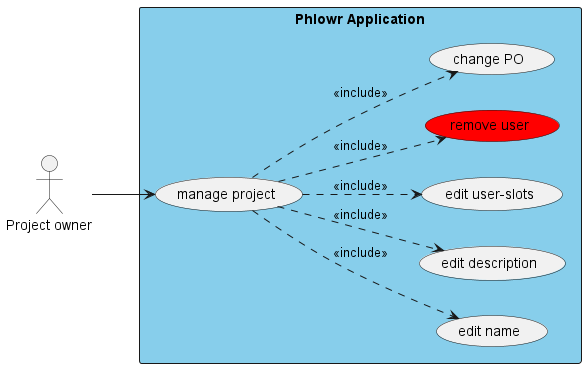
\includegraphics[width=0.3\linewidth]{../content/diagrams/usecase/manageProject/manageProjectUseCaseRemoveUserSelected.png}
      \caption{Use Case Diagaramm <remove user> }
    \end{center}
  \end{figure}

  \begin{table}[H]
    \centering
    \settowidth\tymin{executeIncomingCommand()}
    \setlength\extrarowheight{2pt}
    \begin{tabulary}{1.0\textwidth}{|m{4cm}|m{9cm}|}
      \hline
      \textbf{Use Case} &
      \textbf{REMOVE USER}\\
      \hline
      \textbf{Beschreibung} &
      Ein User wird aus einem Projekt entfernt\\ 
      \hline
      \textbf{Includes} &
      \begin{itemize}
       \item keine
        \end{itemize}\\
        \hline  
      \textbf{Akteure} &
      Projekt-Owner\\ 
      \hline
      \textbf{Auslöser} &
      \begin{itemize}
        \item ein Entwickler arbeitet nicht mehr am Projekt
        \item ein Entwickler hat fälschlicherweise beim Projekt registriert
         \end{itemize}\\  
      \hline
      \textbf{Vorbedingungen} &
      \begin{itemize}
        \item Vorbedingungen vom <manage project>-Use-Case
        \item Der zu entfernende User hat sich als Entwickler beim Projekt registriert
        \item Die vorhandenen Tasks des Users wurden vorgängig bereinigt
      \end{itemize}\\  
      \hline
      \textbf{Abschlussbedingunen} &
      Der User ist nicht mehr im Projekt registriert\\ 
      \hline
      \textbf{Ablauf} &
      \begin{enumerate}
        \item Applikation öffnen
        \item <Projekt Editieren> wählen
        \item unter dem Abschnitt <Entwickler> wird der entsprechende User geöffnet
        \item <Entwickler entfernen> wird gewählt
        \item Speichern
        \end{enumerate}\\ 
      \hline
      \textbf{Zu Beachten / Notizen} &
      \begin{itemize}
        \item wird ein User entfernt, so müssen allfällige Kommentare des Users in den Tasks usw. entsprechend berücksichtigt werden
        \end{itemize}\\ 
      \hline
    \end{tabulary}
    \caption{Use Case: manage project -> remove user}
  \end{table}

   \newpage


  
   %---REGISTER AS DEV USECASE---
   \subsubsection{Als Entwickler registrieren}

\begin{figure}[H]
    \begin{center}
      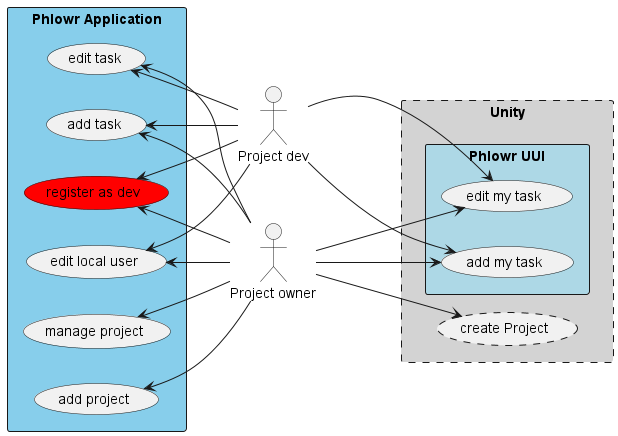
\includegraphics[width=0.3\linewidth]{../content/diagrams/usecase/overview/overviewUseCaseRegisterAsDevSelected.png}
      \caption{Use Case Diagaramm <register as dev> }
    \end{center}
  \end{figure}

   \begin{table}[H]
    \centering
    \settowidth\tymin{executeIncomingCommand()}
    \setlength\extrarowheight{2pt}
    \begin{tabulary}{1.0\textwidth}{|m{4cm}|m{9cm}|}
      \hline
      \textbf{Use Case} &
      \textbf{REGISTER AS DEV}\\
      \hline
      \textbf{Beschreibung} &
      Ein User registriert sich bei einem Projekt.
      Dies ist nötig, damit der User zur Planung im Projekt zu Verfügung steht.\\ 
      \hline
      \textbf{Includes} &
      \begin{itemize}
       \item keine
        \end{itemize}\\ 
        \hline 
      \textbf{Akteure} &
      Entwickler\\ 
      \hline
      \textbf{Auslöser} &
      \begin{itemize}
        \item ein Entwickler möchte an einem Projekt mitarbeiten
         \end{itemize}\\  
      \hline
      \textbf{Vorbedingungen} &
      \begin{itemize}
        \item es ist ein freier Slot im Projekt verfügbar
        \item der Entwickler ist im Projekt noch nicht registriert
        \item das Projekt ist auf dem aktuellsten Stand
      \end{itemize}\\  
      \hline
      \textbf{Abschlussbedingunen} &
      Der User ist im Projekt zur plan verfügbar 
      Der User kann für sich selbst Tasks im Projekt erstellen\\
      \hline
      \textbf{Ablauf} &
      \begin{enumerate}
        \item Applikation öffnen
        \item Projekt öffnen
        \item <Als Entwickler Registrieren> klicken
        \item Speichern
        \item falls nötig Projekt synchronisieren
        \end{enumerate}\\ 
      \hline
      \textbf{Zu Beachten / Notizen} &
      \begin{itemize}
        \item das Projekt muss auf dem neusten Stand sein -> es könnten Merge-Konflikte auftreten
        \end{itemize}\\ 
      \hline
    \end{tabulary}
    \caption{Use Case: register as dev}
  \end{table}

   \newpage


  %---ADD TASK USECASE-TABLE---
  \subsubsection{Task hinzufügen (Applikation)}

\begin{figure}[H]
    \begin{center}
      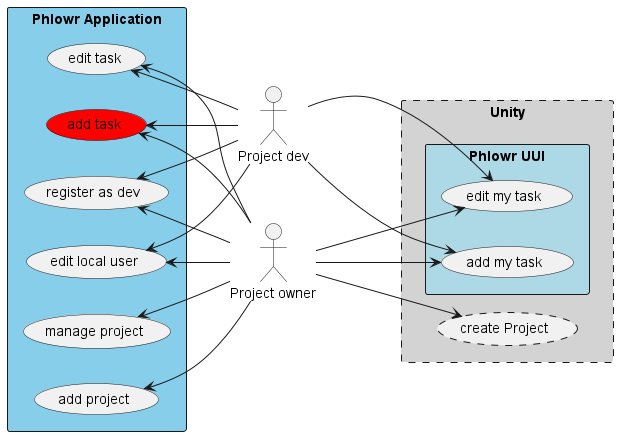
\includegraphics[width=0.25\linewidth]{../content/diagrams/usecase/overview/overviewUseCaseAddTaskSelected.png}
      \caption{Use Case Diagaramm <add Task> }
    \end{center}
  \end{figure}

  \begin{table}[H]
    \centering
    \settowidth\tymin{executeIncomingCommand()}
    \setlength\extrarowheight{2pt}
    \begin{tabulary}{1.0\textwidth}{|m{4cm}|m{9cm}|}
      \hline
      \textbf{Use Case} &
      \textbf{ADD TASK}\\
      \hline
      \textbf{Beschreibung} &
      Ein Task wird dem Projekt hinzugefügt\\ 
      \hline
      \textbf{Includes} &
      \begin{itemize}
       \item keine
        \end{itemize}\\ 
        \hline 
      \textbf{Akteure} &
      \begin{itemize}
       \item Entwickler
       \item Projekt-Owner
        \end{itemize}\\  
        \hline
      \textbf{Auslöser} &
      \begin{itemize}
        \item Ein Task soll dem Projekt hinzugefügt werden
         \end{itemize}\\  
      \hline
      \textbf{Vorbedingungen} &
      \begin{itemize}
        \item Das Projekt ist der Applikation hinzugefügt
        \item Der Ersteller ist Projekt-Owner oder beim Projekt als Entwickler registriert
        \item das Projekt ist auf dem aktuellsten Stand
      \end{itemize}\\  
      \hline
      \textbf{Abschlussbedingunen} &
      Ein neuer Task ist im Projekt verfügbar\\
      \hline
      \textbf{Ablauf} &
      \begin{enumerate}
        \item Applikation öffnen
        \item Projekt öffnen
        \item <Task hinzufügen> klicken
        \item Details des neuen Tasks ausfüllen (Name, Beschreibung usw.)
        \item Speichern
        \item Projekt synchronisieren
        \end{enumerate}\\ 
      \hline
      \textbf{Zu Beachten / Notizen} &
      \begin{itemize}
        \item Tasks können ebenfalls bei bereits existierenden Tasks hinzugefügt werden, dazu wird einfach der entsprechende Task geöffnet.
        \end{itemize}\\ 
      \hline
    \end{tabulary}
    \caption{Use Case: add task}
  \end{table}
 
  \newpage



  %---CLASSSDIAGRAM---
  \newpage
\subsection{Klassendiagramm}
\begin{figure}[H]
  \begin{center}
    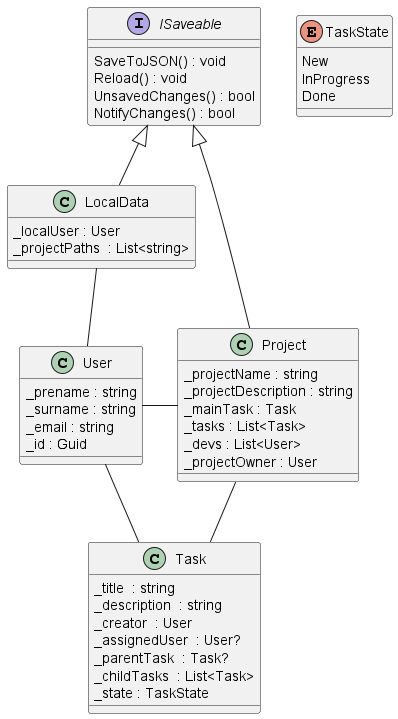
\includegraphics[width=0.5\linewidth]{../content/diagrams/class/classDiagram/classDiagram.png}
    \caption{Klassendiagramm}
  \end{center}
\end{figure}
\subsubsection{Projekt Klassenbeschreibung}
\begin{table}[H]
  \centering
  \settowidth\tymin{executeIncomingCommand()}
  \setlength\extrarowheight{2pt}
  \begin{tabulary}{1.0\textwidth}{|l|l|}
    \hline
    \textbf{Klasse} &
    \textbf{Projekt}\\
    \hline
    \multicolumn{2}{c}{Attribute}\\
    \hline
  \end{tabulary}
  \caption{Klassenbeschreibung: Projekt}
\end{table}


\newpage
\subsection{Sequenzdiagramme}
%---LOAD LOCAL DATA SEQUENCE---
\subsubsection{Laden der lokalen Daten beim Starten der Applikation}
Da alle lokal zu persistierenden Daten in einem JSON-Dokument abgespeichert werden,
müssen diese Daten beim Starten der Applikation geladen werden. Dabei gibt es zwei Szenarien:\\
\begin{enumerate}
  \item Die Applikation wird zum ersten Mal gestartet und es existiert noch kein JSON-Dokument\\
  \item Es existieren bereits gespeicherte Daten in Form eines JSON-Dokuments\\
\end{enumerate}

In der Klasse „LocalData“ wird die statische Methode „LoadOrCreate“ ausgeführt, in dieser Methode wird über
den Data-Access-Layer (DAL) geprüft, ob ein solches JSON Dokument existiert. Existiert dieses, so wird
das Objekt über den DAL ausgelesen, dabei enthält das Objekt ebenfalls eine Instanz der Klasse „LocalUser“
welcher somit ebenfalls geladen wurde.\\
Existiert kein JSON-Dokument so wird erst ein neuer User als „LocalUser“ erstellt, dabei wird auch dessen Guid generiert
(Das Generieren der Guid eines Users darf nur hier erfolgen!). Anschliessend wird eine neue Instanz der Klasse „LocalData“ mit dem neuen „LocalUser“ erstellt.
Diese wird über den DAL als JSON-Dokument abgespeichert und kann beim nächstmaligen Starten der Applikation geladen werden.

\begin{figure}[H]
  \begin{center}
    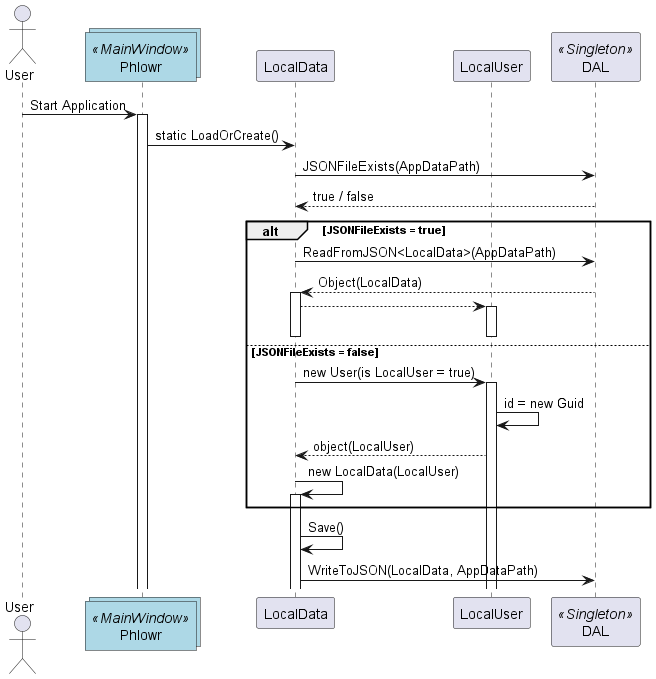
\includegraphics[width=0.7\linewidth]{../content/diagrams/sequence/loadLocalDataSequence/loadLocalDataSequence.png}
    \caption{Sequenzdiagramm: Load LocalData}
  \end{center}
\end{figure}
\newpage

%---ADD PROJECT SEQUENCE---
\subsubsection{Projekt Hinzufügen}
Das Hinzufügen eines Projektes ist sehr einfach gehalten, denn bei diesem Vorgang werden keine Projekt-Objekte erzeugt oder geladen.
Durch einen Klick auf „Projekt hinzufügen“ wird der Verzeichnis-Explorer angezeigt, in diesem navigiert der Benutzer zum gewünschten Unity-Projektordner
und wählt diesen aus. Anschliessend wird die Methode „AddProjectPath“ in der LocalData-Instanz ausgeführt, ist der Pfad nicht bereits vorhanden, so wird dieser in die Liste aufgenommen.\\
Zum Schluss wird die LocalData-Instanz wieder abgespeichert.\\
Das Erzeugen der Projekte wird im Sequenzdiagramm „Laden der Projekte“ behandelt.
\begin{figure}[H]
  \begin{center}
    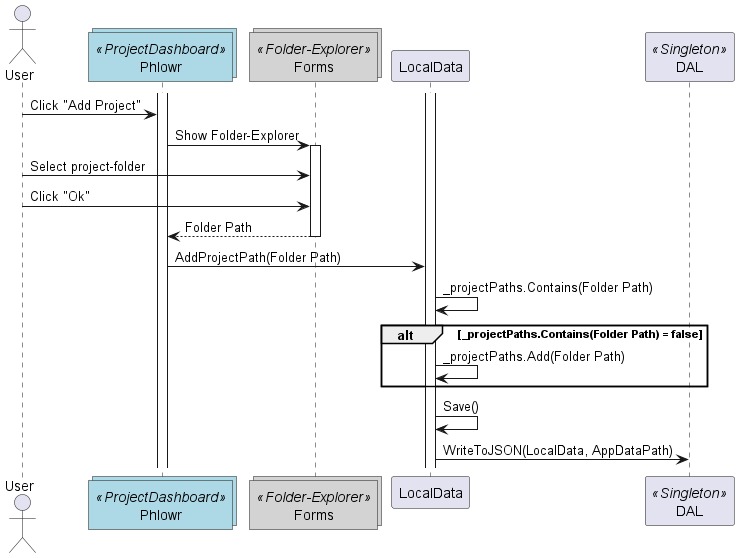
\includegraphics[width=0.7\linewidth]{../content/diagrams/sequence/addProjectSequence/addProjectSequence.png}
    \caption{Sequenzdiagramm: Add Project}
  \end{center}
\end{figure}
\newpage

%---LOAD PROJECTS SEQUENCE---
\subsubsection{Laden der Projekte}
Beim Öffnen des Projekt-Dashboards werden alle hinzugefügten Projekte geladen.\\
Dafür wird durch alle Projekt-Pfade, welche in der LocalData-Instanz vorhanden sind, geloopt. Für jeden Pfad wird die statische Methode „LoadOrCreate“ in der Projekt-Klasse ausgeführt.
Diese Methode überprüft über den DAL, ob bereits ein JSON-Dokument unter dem angegebenen Pfad vorhanden ist.
Ist ein JSON-Dokument vorhanden, so wird dieses über den DAL geladen und zurückgegeben. Ist noch keine Projektdatei vorhanden, so wird eine neue Projekt-Instanz erzeugt, 
der Projekt-Owner der neu erzeugten Instanz wird automatisch der LocalUser. Die Instanz wird anschliessend abgespeichert, als JSON-Dokument im angegebenen Pfad abgelegt und zurückgegeben.
Das Projekt-Dashboard fügt die erhaltene Projekt-Instanz zur Projekt-Liste hinzu.
\begin{figure}[H]
  \begin{center}
    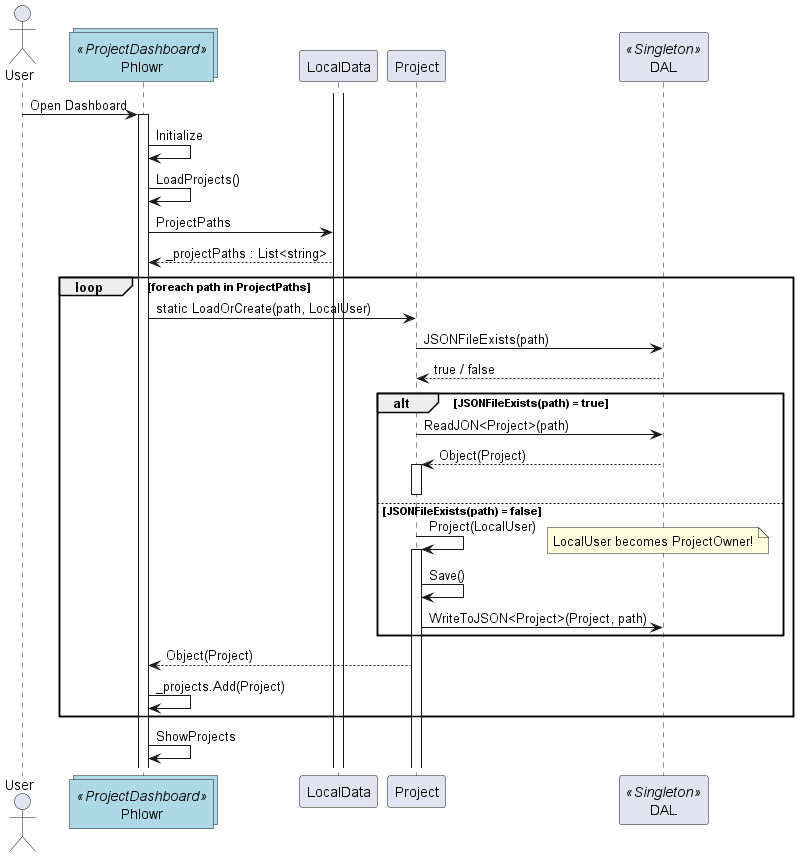
\includegraphics[width=0.7\linewidth]{../content/diagrams/sequence/loadProjectsSequence/loadProjectsSequence.png}
    \caption{Sequenzdiagramm: Load Projects}
  \end{center}
\end{figure}
\newpage

%---REGISTER AS USER SEQUENCE---
\subsubsection{Als Entwickler registrieren}
Damit ein User als Entwickler in einem Projekt geplant werden kann, muss er sich zuerst beim Projekt registrieren.
Dafür navigiert er zum entsprechenden Projekt und wählt „Als Entwickler registrieren“ aus. Dadurch wird auf der entsprechenden Projekt-Instanz
die Methode „RegisterUser“ mit dem LocalUser als Übergabeparameter ausgeführt.\\
In dieser Methode wird überprüft, ob noch ein freier Slot verfügbar ist und ob sich der User nicht schon registriert hat. 
Für letzteres wird über alle registrierten User zusätzlich nach der Guid des neuen Users gesucht.
\begin{figure}[H]
  \begin{center}
    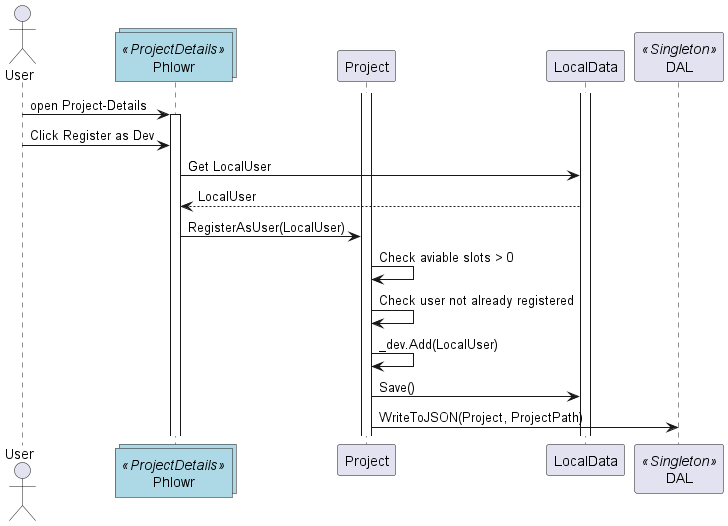
\includegraphics[width=0.7\linewidth]{../content/diagrams/sequence/registerAsUserSequence/registerAsUserSequence.png}
    \caption{Sequenzdiagramm: Register as user}
  \end{center}
\end{figure}
\newpage

\subsection{State Diagramme}
\newpage
\subsection{Systemarchitektur}
\newpage
\subsection{Mockup}
